\item A horizontal smooth rod \( AB \) rotates with a constant angular velocity \( \omega = 2.00 \ \text{rad/s} \) about a vertical axis passing through its end \( A \). A freely sliding sleeve of mass \( m = 0.50 \ \text{kg} \) moves along the rod from the point \( A \) with the initial velocity \( v_0 = 1.00 \ \text{m/s} \). Find the Coriolis force acting on the sleeve (in the reference frame fixed to the rotating rod) at the moment when the sleeve is located at the distance \( r = 50 \ \text{cm} \) from the rotation axis.
    \begin{center}
        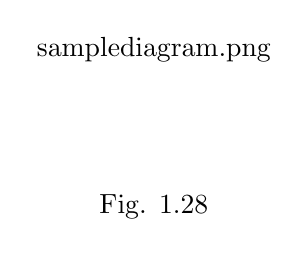
\begin{tikzpicture}
            \node at (0, 0) {{samplediagram.png}};
            \node at (0, -2) {Fig. 1.28};
        \end{tikzpicture}
    \end{center}\begin{solution}
    
    \begin{align*}
        \intertext{The sleeve is free to slide along the rod $AB$. Thus the centrifugal force acts on it in the outward direction along the river.}
        m\omega' &= m\omega^2 r \\
        \intertext{where}
        v' &= \frac{dr}{dt} \\
        \intertext{But,}
        w' &= \frac{vdv}{dr} = \frac{d}{dr} \left( \frac{1}{2} v^2 \right)
    \end{align*}

    \begin{align*}
        \intertext{So,}
        \frac{1}{2} v^2 &= \frac{1}{2} \omega^2 r^2 + \text{constant} \\
        \intertext{or}
        v^2 &= v_0^2 + \omega^2 r^2 \\
        \intertext{$v_0$ being the initial velocity when $r = 0$. The Coriolis force is then}
        2m\omega\sqrt{v_0^2 + \omega^2 r^2} &= 2m\omega r \sqrt{1 + \frac{v_0^2}{\omega^2 r^2}} = 2.83 \ \text{N \ (on substituting values)}
    \end{align*}
    
\end{solution}